% ****** Start of file apssamp.tex ******
%
%   This file is part of the APS files in the REVTeX 4.1 distribution.
%   Version 4.1r of REVTeX, August 2010
%
%   Copyright (c) 2009, 2010 The American Physical Society.
%
%   See the REVTeX 4 README file for restrictions and more information.
%
% TeX'ing this file requires that you have AMS-LaTeX 2.0 installed
% as well as the rest of the prerequisites for REVTeX 4.1
%
% See the REVTeX 4 README file
% It also requires running BibTeX. The commands are as follows:
%
%  1)  latex apssamp.tex
%  2)  bibtex apssamp
%  3)  latex apssamp.tex
%  4)  latex apssamp.tex
%
%\documentclass[twocolumn,prl,11pt,a4paper]{revtex4}

\documentclass[%
%12pt,
reprint11,
%superscriptaddress,
%groupedaddress,
%unsortedaddress,
%runinaddress
%frontmatterverbose, 
%preprint,
%showpacs,preprintnumbers,
%nofootinbib,
%nobibnotes,
%bibnotes,
 amsmath,amssymb,
 aps,
%pra,
%prb,
%rmp,
%prstab,
%prstper,
%floatfix,
]{revtex4-1}
\usepackage{wrapfig}
\usepackage{caption}
\usepackage{subfig}
\usepackage{amssymb}
\setcounter{tocdepth}{3}
\usepackage{graphicx}
\usepackage[]{caption}	
\usepackage{amsmath}
\usepackage{multirow}
\usepackage{booktabs}
\usepackage{url}
\usepackage{epstopdf}
\usepackage{tabularx}
\usepackage[T1]{fontenc}
\usepackage[utf8]{inputenc}
%\usepackage{floatrow}
\usepackage{dcolumn}% Align table columns on decimal point
\usepackage{bm}% bold math
%\usepackage{hyperref}% add hypertext capabilities
%\usepackage[mathlines]{lineno}% Enable numbering of text and display math
%\linenumbers\relax % Commence numbering lines

%\usepackage[showframe,%Uncomment any one of the following lines to test 
%%scale=0.7, marginratio={1:1, 2:3}, ignoreall,% default settings
%%text={7in,10in},centering,
%%margin=1.5in,
%%total={6.5in,8.75in}, top=1.2in, left=0.9in, includefoot,
%%height=10in,a5paper,hmargin={3cm,0.8in},
%]{geometry}

\begin{document}

\title{A Space-Efficient Design for a Reversible Floating Point Adder\\ in Quantum Computing} %Title of paper

% repeat the \author .. \affiliation  etc. as needed
% \email, \thanks, \homelpage, \altaffiliation all apply to the current author.
% Explanatory text should go in the []'s, 
% actual e-mail address or url should go in the {}'s for \email and \homepage.
% Please use the appropriate macro for the type of information

% \affiliation command applies to all authors since the last \affiliation command. 
% The \affiliation command should follow the other information.

\author{ Trung Duc Nguyen
}
\author{ Rodney Van Meter
}
%\email[]{deplop@sfc.wide.ad.jp}
%\homepage[]{Your web page}
%\thanks{}
%\altaffiliation{}
\affiliation{Keio University, Faculty of Environment and Information Studies, 5322 Endo, Fujisawa, Kanagawa, Japan}

% Collaboration name, if desired (requires use of superscriptaddress option in \documentclass). 
% \noaffiliation is required (may also be used with the \author command).
%\collaboration{}
%\noaffiliation
\begin{abstract}
%\boldmath
  There are few existing designs for reversible floating-point adders
  and none suitable for quantum computation. In this paper we propose
  a space-efficient reversible floating-point adder, suitable for
  binary quantum computation, improving the design of Nachtigal et
  al.~\cite{nachtigal}. Our work focuses on improving the reversible
  designs of the alignment unit and the normalization unit, which are
  the most expensive parts. By changing a few elements of the existing
  algorithm, we have reduced the cost about 68\% compared to the
  existing design. We also propose fault-tolerant designs. The KQ for
  our fault-tolerant design is almost sixty times as expensive as for
  a 32-bit fixed-point addition. We note that the floating-point
  representation makes in-place, truly reversible arithmetic
  impossible, requiring us to retain both inputs, which limits the
  sustainability of its use for quantum computation.

\keywords{reversible circuit, quantum computing, low-power computing, nano technology, IEEE-754 specification} 
\end{abstract}
%\pacs{}% insert suggested PACS numbers in braces on next line

\maketitle %\maketitle must follow title, authors, abstract and \pacs
\bibliographystyle{plain}
% Body of paper goes here. Use proper sectioning commands. 
% References should be done using the \cite, \ref, and \label commandsa


%\section{Introduction}


\par Computer arithmetic is generally carried out as either integer
arithmetic, more correctly called fixed-point arithmetic in most
contexts, or floating point arithmetic. Floating point numbers, as the
name implies, allow the decimal (binary) point to be repositioned
according to the value of an exponent. Fixed point numbers are limited
to the range $-2^n..2^n-1$ for an $n$-bit number, but a floating point
can cover many more orders of magnitude. The price for this
flexibility is reduced precision within the same storage space, as
some bits are dedicated to storing the exponent, and substantially
higher execution costs. However, floating point is the standard
representation for scientific data, as data points often span a broad
dynamic range or a range that is difficult to determine \emph{a
  priori}.

\par Some quantum algorithms would benefit from the availability of a
library of floating point operations. Algorithms that focus on
physical phenomena, such as quantum
chemistry~\cite{brown10:q-sims-entropy,kassal11:qchem-sim-review} and
quantum field theory calculations~\cite{jordan12:qa-qft}, seem
especially likely to be able to take advantage of this
capability. Implementations of Harrow, Hassidim and Lloyd's algorithm
for linear systems~\cite{clader2013quantum,harrow:lineqs} and Jozsa's
variant of Hallgren's algorithm that uses real numbers may also
benefit~\cite{jozsa2003notes}.

\par While many fixed point adder designs have been introduced, we are
aware of only one design for a reversible floating-point quantum
adder, by Nachtigal, Thapliyal and Ranganathan (NTR), and this design
is expensive~\cite{nachtigal}. Our proposed design eliminates about
68\% of the cost. Moreover, the NTR design as presented leaves many
temporary variables in a dirty state, making it unsuitable as-is for
quantum computing; our design reduces this number and shows how to
compose this design in a fully-reversible setup.

\par A truly reversible circuit generally calculates $ \langle A,B
\rangle \xrightarrow{U} \langle A,f(A,B) \rangle $ where each element
of the tuple is a fixed-size register and $U$ is a unitary operation
that realizes $f(A,B)$. Nachtigal's circuit actually calculates $
\langle A,B,0,0 \rangle \xrightarrow{U} \langle A,B,A+B,G \rangle$
where $A$, $B$ and $A+B$ are single precision floating point numbers
and $G$ is a large amount of ancillary data left in a garbage
state. We adapt Bennett's original reversible formulation,
\begin{align}
   \langle A,B,0,0,0 \rangle \xrightarrow{U} & \langle A',B',f(A,B),G,0 \rangle \\\nonumber
   \xrightarrow{CNOT} & \langle A',B',f(A,B),G,f(A,B) \rangle  \\\nonumber
   \xrightarrow{U^\dag} & \langle A,B,0,0,f(A,B) \rangle 
\label{eqn:Benett}
\end{align}
to complete the reversibility and make the circuit suitable for quantum computation.

\par This cannot solve the fundamental problem that floating point
addition is not 1:1, requiring us to retain both inputs as well as the
output. Thus, quantum circuits that require many floating point
operations may result in unsustainable growth of memory resources.

In quantum computing we often use KQ~\cite{fault-tolerant} as the cost
metric, which helps to calculate the demands on quantum error
correction. KQ is calculated by multiplying the number of qubits used
and the circuit depth.  Table~\ref{tab:T-depth} shows the $T$-depth of
each stage.  The total KQ for the whole architecture is 723,301. This
compares to a KQ for a 32-bit CDKM ripple-carry adder of
12,474~\cite{cuccaro04:new-quant-ripple}. A floating-point addition is
thus nearly sixty times as expensive as fixed-point.

\begin{table}
\centering
\begin{tabular}{|c|c|}
\hline
\textbf{Stage} & \textbf{$T$-depth} \\
\hline
 Swap & 174  \\ \hline
 Alignment & 194  \\ \hline
 Addition &  57 \\ \hline
 Conversion & 212  \\ \hline
 Normalization & 244  \\ \hline
 Rounding & 0 \\ \hline 
 Total &  881 \\ \hline 
\end{tabular}
\\
\caption{$T$-depth of each stage in our fault-tolerant adder.}
\label{tab:T-depth}
\end{table} 

% \section{Floating-Point Addition}

The basics of a floating-point adder algorithm will be briefly
summarized with attention to the demands of reversibility. Two 32-bit
IEEE-754 single-precision floating-point numbers $A$ and $B$ are to be
added. Before two numbers can be added, they must be aligned.  The
smaller number's exponent is incremented until its exponent reaches
the larger number's, in conjunction with shifting the smaller number's
mantissa to the right. Once the exponents are equal, the mantissas can
be summed. The sum is normalized and rounded at the
end. Fig.~\ref{fig:overview} shows the general algorithm adapted to
show constant inputs and garbage outputs. The garbage outputs are
eventually cleaned by reversing this circuit using Bennett's method.

\begin{figure}[h]
\centering
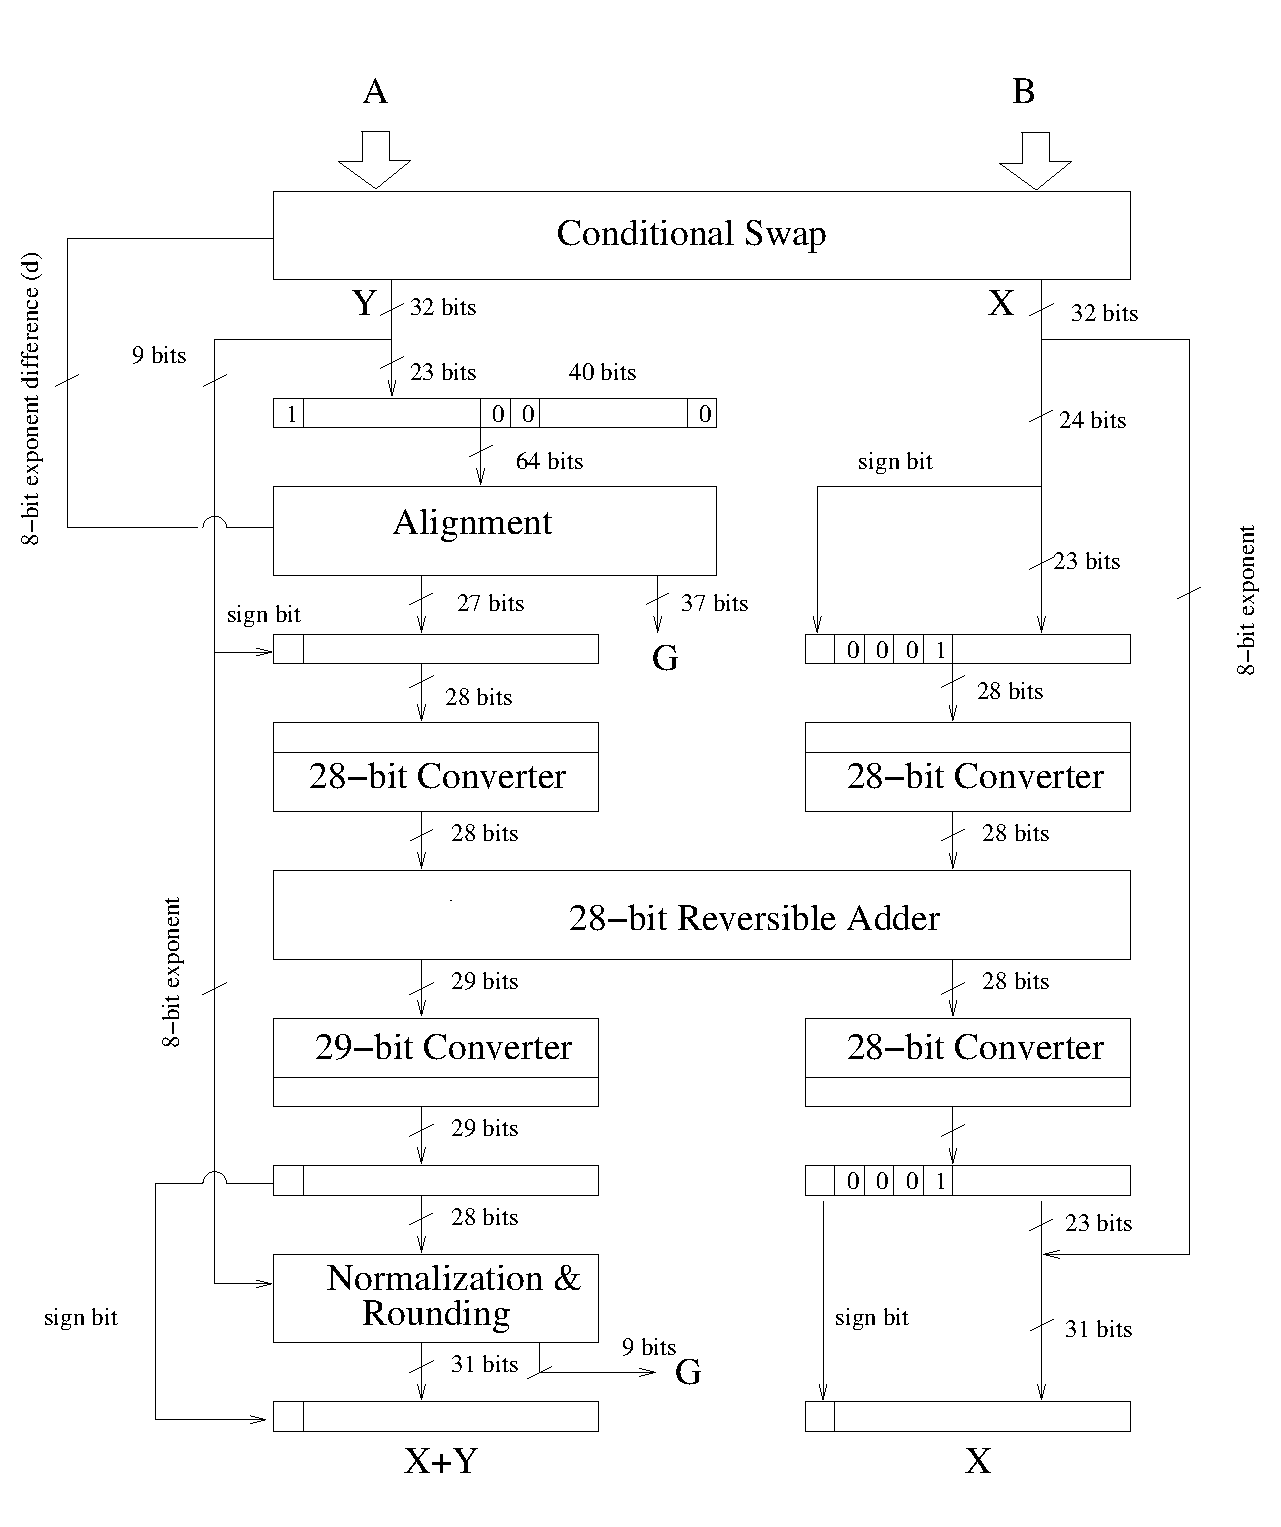
\includegraphics[width=7cm]{algorithm.eps}
%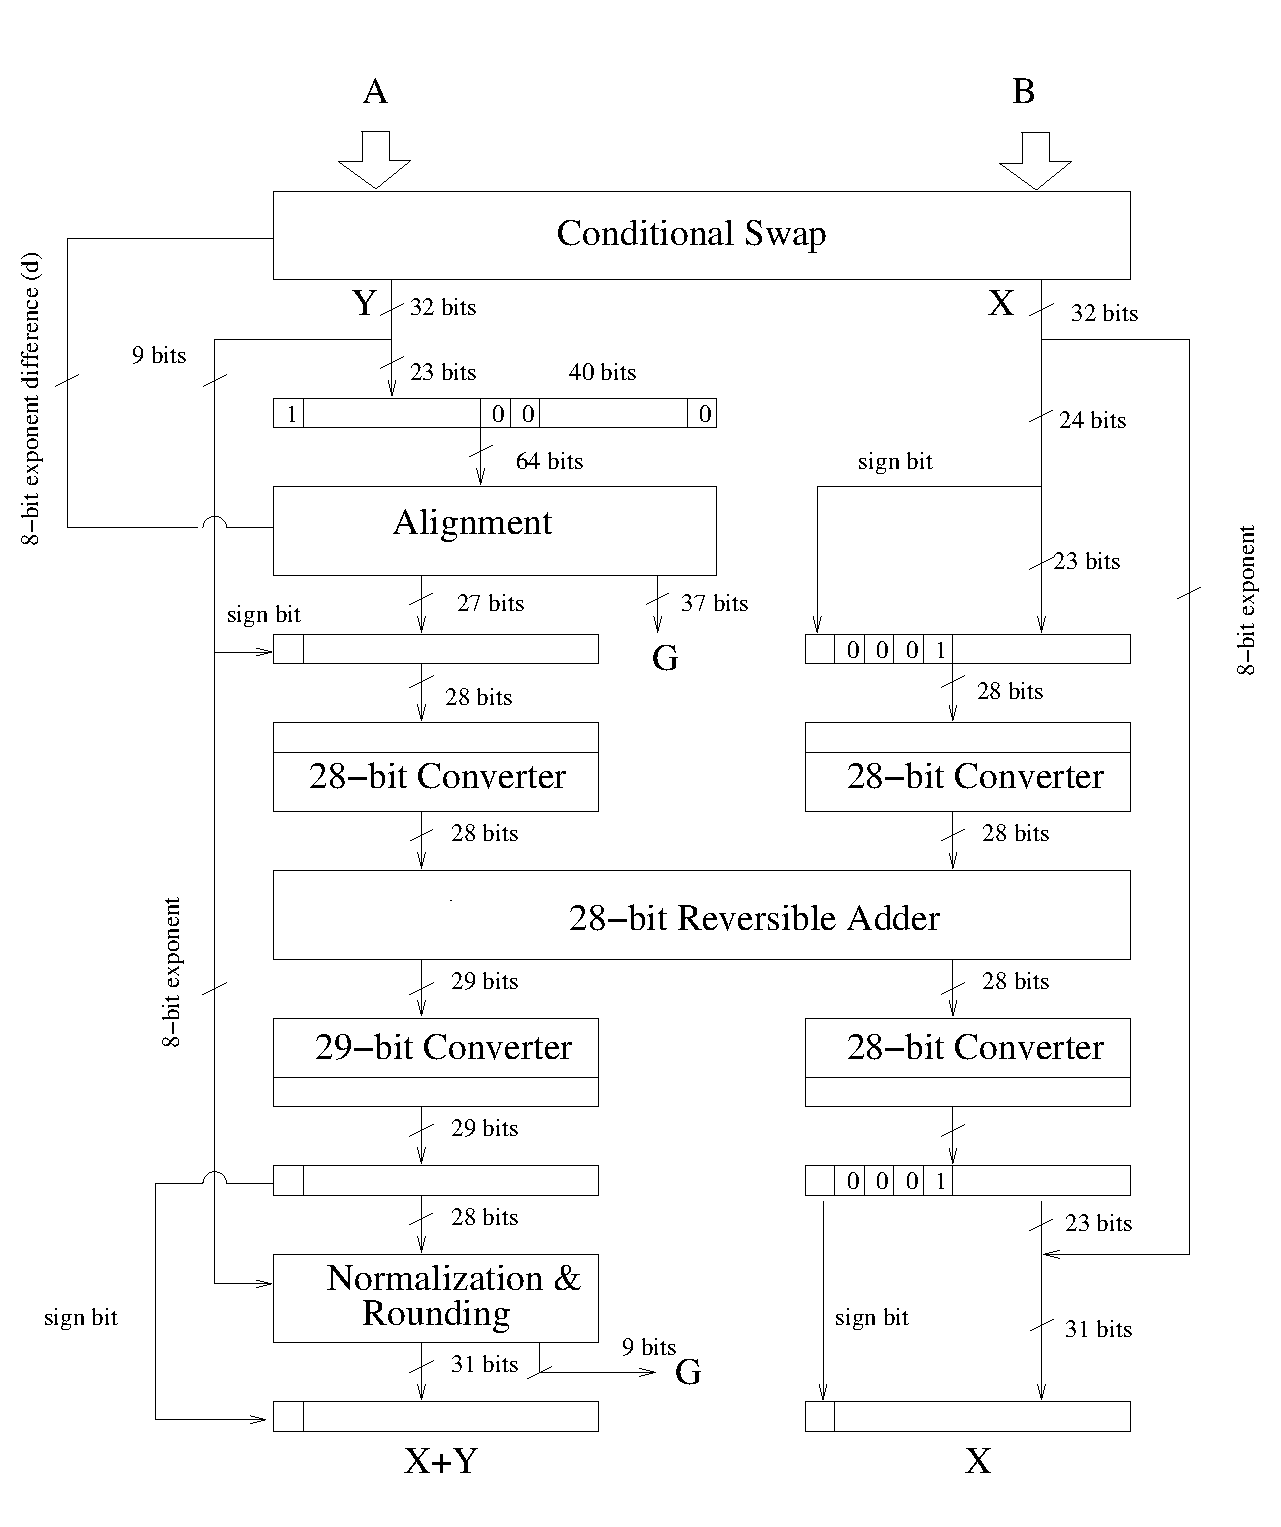
\includegraphics[width=1\textwidth]{algorithm.eps}
\caption{Overview of our floating point adder.}
\label{fig:overview}
\end{figure}

\par At this stage of the execution, the system state corresponds to
$\langle A',B',f(A,B),G \rangle $. To complete the reversibility of
the circuit, we must bring in an additional 32-bit register, execute
transverse CNOTs from the output value, then run our complete circuit
in reverse to clean up all of the garbage as shown in Eq. (1). Thus,
the complete circuit uses 821 qubits: 64 variable input qubits and 757
input ancillae. On output, most ancillae are returned to their
pristine state, but 32 have been drafted into permanent use. We
conclude that floating point addition is not a ``green" operation,
unsustainable with repeated use.

\bibliography{duc-bib}% Produces the bibliography via BibTeX.

\end{document}
%
% ****** End of file apssamp.tex ******
{\bf Reversible Conditional Swap}  A reversible conditional swap is necessary because we need to figure out which number has the smaller exponent and then input it to the reversible alignment step. If expA $<$ expB (expA stands for the exponent of A) then swap the two numbers, otherwise do nothing. After this step, the number with the smaller exponent always comes out in the Y output, which connects to the reversible barrel shifter~\cite{barrel-shifter} in the next step.  

{\bf Reversible Alignment}
We need reversible alignment because we can only add two mantissas when the two exponents are equal, so we need a reversible shifter. The shifted amount is the difference between the two exponents. Because the IEEE-754 floating-point single-precision specification uses an 8-bit exponent, the difference of the exponents is up to 256. Thus, a (256, 8) reversible barrel shifter (256 input bits, 8 control lines)~\cite{efficient-barrel} is used in the NTR design. This is one of the key reasons for the large quantum cost, constant input and garbage output of the NTR design. Our design significantly reduces this cost. 
\par The IEEE-754 specification also requires three extra bits as described above. Thus, we need a sticky bit cascade unit to calculate the sticky bit after shifting. The sticky bit is calculated ORing together the $27^{th}$ to $256^{th}$ bits. 

{\bf Two's complement Conversion and Reversible Addition}
The IEEE-754 specification represents numbers in sign-magnitude format (1 sign bit, 23 mantissa bits). To add two mantissas after the alignment step, the two numbers will be represented in two's complement format. After the addition, the result will be converted back to sign-magnitude format. Thus, we need \emph{sign-magnitude to two's complement} reversible converters and \emph{two's complement to sign-magnitude} reversible converters before and after the addition. The proposed converter will be described later. After the \emph{sign-magnitude to two's complement} conversion, the addition is done by a reversible adder which is constructed from 27 RFA (Reversible Full Adder) gates and one RHA (Reversible Half Adder) gate. 


{\bf Reversible Normalization and Rounding}
After the addition, the result may have a number of leading zero bits or have one more bit with value of one at the most significant bit (MSB). The normalization is need to adjust the result so that it conforms to the floating-point number format. In normalization, if a shift is required, it is either a one place right shift or a multiple-place left shift. If the MSB has a value of one, one place of right shift takes place and the 8-bit exponent is passed through a reversible conditional increment unit. Otherwise, one or several places of left shift is needed in conjunction with a corresponding decrement of the 8-bit exponent. 

{\bf Discussion and Conclusion}
With improvements in the two most hardware-intensive parts, this proposed design has reduced the quantum cost by 68\%, the number of garbage outputs by 72\% and the number of constant inputs by 71.5\%. We also give a fault-tolerant version of the whole architecture.
